\begin{figure}
	\centering
	\pgfplotsset{every axis legend/.append style={
		at={(1.05,0.5)},
		anchor=west}}
	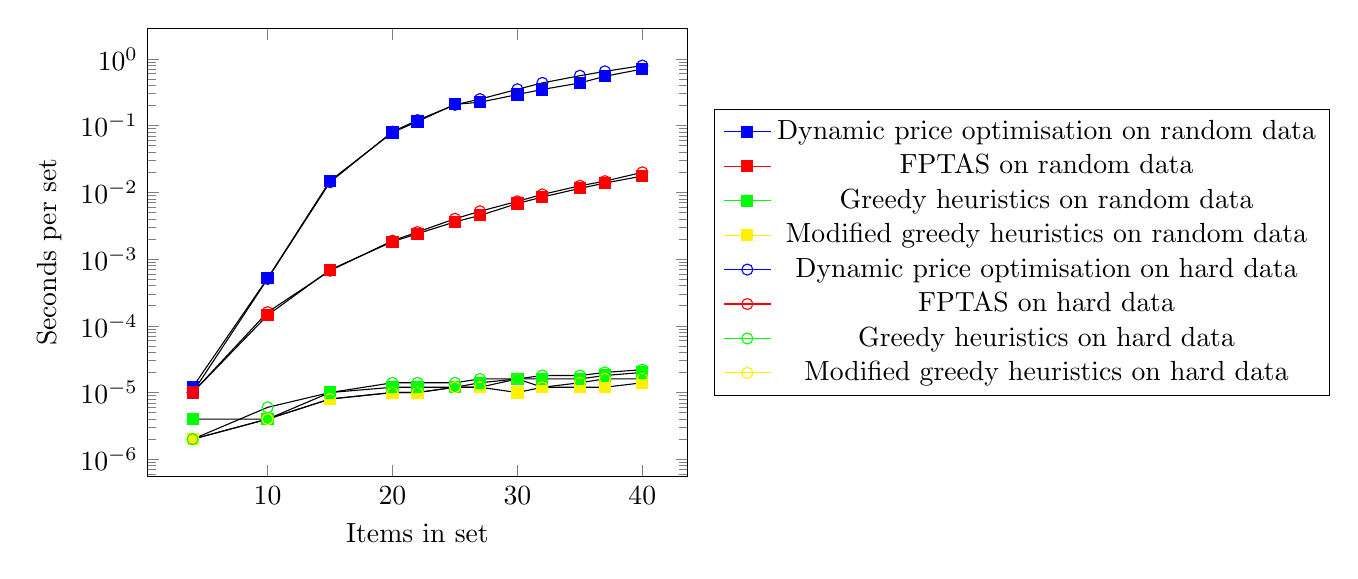
\begin{tikzpicture}
		\begin{semilogyaxis}[
			xlabel=Items in set,
			ylabel=Seconds per set,
			scatter/classes={
				dynN={mark=square*,blue},
				fptasN={mark=square*,red},
				singleN={mark=square*,green},
				hungryN={mark=square*,yellow},
				dynH={mark=o,blue},
				fptasH={mark=o,red},
				singleH={mark=o,green},
				hungryH={mark=o,yellow}
				}
			]
			\addplot[scatter,%
				scatter src=explicit symbolic]%
			table[meta=label] {
				x y label
				4 .000012 dynN
				10 .000514 dynN
				15 .014872 dynN
				20 .078888 dynN
				22 .114784 dynN
				25 .208052 dynN
				27 .223608 dynN
				30 .291732 dynN
				32 .348044 dynN
				35 .434604 dynN
				37 .547092 dynN
				40 .704324 dynN
			};
			\addplot[scatter,%
				scatter src=explicit symbolic]%
			table[meta=label] {
				x y label
				4 .000010 fptasN
				10 .000144 fptasN
				15 .000690 fptasN
				20 .001822 fptasN
				22 .002398 fptasN
				25 .003606 fptasN
				27 .004508 fptasN
				30 .006790 fptasN
				32 .008502 fptasN
				35 .011454 fptasN
				37 .013754 fptasN
				40 .017528 fptasN
			};
			\addplot[scatter,%
				scatter src=explicit symbolic]%
			table[meta=label] {
				x y label
				4 .000002 hungryN
				10 .000004 hungryN
				15 .000008 hungryN
				20 .000010 hungryN
				22 .000010 hungryN
				25 .000012 hungryN
				27 .000012 hungryN
				30 .000010 hungryN
				32 .000012 hungryN
				35 .000012 hungryN
				37 .000012 hungryN
				40 .000014 hungryN
			};
			\addplot[scatter,%
				scatter src=explicit symbolic]%
			table[meta=label] {
				x y label
				4 .000004 singleN
				10 .000004 singleN
				15 .000010 singleN
				20 .000012 singleN
				22 .000012 singleN
				25 .000012 singleN
				27 .000014 singleN
				30 .000016 singleN
				32 .000016 singleN
				35 .000016 singleN
				37 .000018 singleN
				40 .000020 singleN
			};
			\addplot[scatter,%
				scatter src=explicit symbolic]%
			table[meta=label] {
				x y label
				4 .000010 dynH
				10 .000504 dynH
				15 .014208 dynH
				20 .080942 dynH
				22 .120590 dynH
				25 .204710 dynH
				27 .249138 dynH
				30 .349580 dynH
				32 .435896 dynH
				35 .558234 dynH
				37 .649110 dynH
				40 .792216 dynH
			};
			\addplot[scatter,%
				scatter src=explicit symbolic]%
			table[meta=label] {
				x y label
				4 .000010 fptasH
				10 .000160 fptasH
				15 .000668 fptasH
				20 .001884 fptasH
				22 .002534 fptasH
				25 .004014 fptasH
				27 .005196 fptasH
				30 .007330 fptasH
				32 .009300 fptasH
				35 .012524 fptasH
				37 .014686 fptasH
				40 .019922 fptasH
			};
			\addplot[scatter,%
				scatter src=explicit symbolic]%
			table[meta=label] {
				x y label
				4 .000002 hungryH
				10 .000004 hungryH
				15 .000008 hungryH
				20 .000010 hungryH
				22 .000010 hungryH
				25 .000012 hungryH
				27 .000012 hungryH
				30 .000016 hungryH
				32 .000012 hungryH
				35 .000014 hungryH
				37 .000016 hungryH
				40 .000016 hungryH
			};
			\addplot[scatter,%
				scatter src=explicit symbolic]%
			table[meta=label] {
				x y label
				4 .000002 singleH
				10 .000006 singleH
				15 .000010 singleH
				20 .000014 singleH
				22 .000014 singleH
				25 .000014 singleH
				27 .000016 singleH
				30 .000016 singleH
				32 .000018 singleH
				35 .000018 singleH
				37 .000020 singleH
				40 .000022 singleH

			};
			\addlegendentry{Dynamic price optimisation on random data}
			\addlegendentry{FPTAS on random data}
			\addlegendentry{Greedy heuristics on random data}
			\addlegendentry{Modified greedy heuristics on random data}
			\addlegendentry{Dynamic price optimisation on hard data}
			\addlegendentry{FPTAS on hard data}
			\addlegendentry{Greedy heuristics on hard data}
			\addlegendentry{Modified greedy heuristics on hard data}
		\end{semilogyaxis}
	\end{tikzpicture}
\caption{Time needed depending on number of items in set}
\label{plot:fullTime}
\end{figure}
